\documentclass{article}

\usepackage[a4paper, left=1.5cm, right=1.5cm, top=2cm, bottom=2cm]{geometry}

\usepackage{amsmath,amssymb}

\usepackage{../../../../components/mathtex}

\usepackage{hyperref}
\usepackage{fancyhdr}
\usepackage{ccicons}
\usepackage{caption}


% Configuration des en-têtes et pieds de page
\pagestyle{fancy}
\fancyhf{} % reset tout

\fancyhead[L]{DL3 Math-Info CD5}
\fancyhead[C]{Topologie}
\fancyhead[R]{2026-2027}

\fancyfoot[L]{Ewen Rodrigues de Oliveira\\\ccbyncsa}
\fancyfoot[R]{\thepage}

\begin{document}

\docTitle{Chapitre 1 : Topologie des espaces vectoriels normés\footnote{Ce chapitre peut être vu comme un sous-chapitre du \href{https://www.ewenrdo.fr/ressources?slug=analyse-3-chapitre-4-topologie-des-espaces-metriques}{Chapitre 4 : Topologie des espaces métriques et des espaces vectoriels normés} du cours Analyse 3.}}

\noindent Dans tout ce chapitre, on note $(E, \langle \cdot, \cdot \rangle)$ un espace préhilbertien\footnote{Voir le \href{https://www.ewenrdo.fr/ressources?slug=calcul-differentiel-5-chapitre-0-espaces-prehilbertiens}{Chapitre 0 : Espaces préhilbertiens}{ sur les espaces préhilbertiens} du cours Calcul différentiel 5} sur $\mathbb{K}$, où $\mathbb{K} = \mathbb{R}$ ou $\mathbb{C}$.
\section{Espaces vectoriels normés}

\subsection{Cadre général}

\definition{
    Une norme $N$ sur $E$ est une application $\| \cdot \| \colon E \to \mathbb{R}_+$ qui vérifie les axiomes suivants :
    \begin{enumerate}
        \item $\forall u \in E, \forall \lambda \in \mathbb{K}, \|\lambda u\| = |\lambda| \cdot \|u\|$ (homogénéité)
        \item $\forall (u,v) \in E^2, \|u+v\| \leq \|u\| + \|v\|$ (inégalité triangulaire)
        \item $\forall u \in E, \|u\| = 0 \Leftrightarrow u = 0_E$ (séparation)
    \end{enumerate}
}
\vocabulary{On dit que le couple $(E, \| \cdot \|)$ est un \textbf{espace vectoriel normé}. Il est commun d'écrire $e.v.n.$.}
\remark{Le dernier point s'appelle séparation car il permet de séparer les vecteurs, c'est-à-dire de savoir si deux vecteurs sont égaux ou non, en calculant $\|u-v\|$.}
\definition{
    Soit $(E, \langle \cdot, \cdot \rangle)$ un espace préhilbertien. On dit que la norme $\| \cdot \|$ est \textbf{associée} au produit scalaire $\langle \cdot, \cdot \rangle$ si :
    $$\|x\| = \sqrt{\langle x, x \rangle}$$
    pour tout $x \in E$.
}

\example{Voici quelques normes qu'il convient de connaître sur $\mathbb{K}^n$ :
\begin{itemize}
    \item La norme $1$ : $\|x\|_1 = \sum_{i=1}^n |x_i|$,
    \item La norme $2$ (euclidienne) : $\|x\|_2 = \sqrt{\sum_{i=1}^n |x_i|^2} = \sqrt{\langle x, x \rangle}$ (c'est la norme associée au produit scalaire canonique),
    \item La norme $\infty$ : $\|x\|_\infty = \max_{1 \leq i \leq n} |x_i|$.
\end{itemize}
}


\example{Sur $E = \mathcal{C}([0,1], \mathbb{K})$, les normes suivantes sont à connaître :
\begin{itemize}
    \item La norme $1$ : $\|f\|_1 = \int_0^1 |f(t)|dt$,
    \item La norme $2$ : $\|f\|_2 = \sqrt{\int_0^1 |f(t)|^2 dt}$,
    \item La norme $\infty$ : $\|f\|_\infty = \max_{t \in [0,1]} |f(t)|$.
\end{itemize}
Elles sont bien définies car $f$ est continue \textit{(il faut le dire en examen !)}.
}

\newpage

\training{Démontrer que la norme $\| \cdot \|_1$ est une norme sur $\mathcal{C}([0,1], \mathbb{K})$.}
\noindent\carreaux{5}

\theorem{Théorème}{Inégalité de Cauchy-Schwarz}{false}{
    Soit $(E, \langle \cdot, \cdot \rangle)$ un espace préhilbertien. Alors pour tous $u,v \in E$, on a :
    $$|\langle u, v \rangle| \leq \|u\| \cdot \|v\|$$
}
\ndlr{cf. Laurent pour la preuve.}

\training{À l'aide de l'inégalité de Cauchy-Schwarz, démontrer que la $\| \cdot \|_2$ est une norme sur $\mathbb{K}^n$.}
\noindent \carreaux{5}

\theorem{Corollaire}{Inégalité triangulaire de la norme}{false}{
    Soit $(E, \langle \cdot, \cdot \rangle)$ un espace préhilbertien. Alors pour tous $u,v \in E$, on a :
    $$\|u+v\| \leq \|u\| + \|v\|$$
}
\noindent{\textbf{Preuve :} Soient $u,v \in E$. On a $\| u+ v \|^2 = \|u\|^2 + 2 \Re(\langle u, v \rangle) + \|v\|^2 \leq \|u\|^2 + 2 |\langle u, v \rangle| + \|v\|^2 \leq \|u\|^2 + 2 \|u\|\|v\| + \|v\|^2 = (\|u\| + \|v\|)^2$. 
En prenant la racine carrée, on obtient l'inégalité triangulaire. $\hfill \square$}


\theorem{Proposition}{Inégalité triangulaire inverse}{false}{
    Soit $(E, \| \cdot \|)$ un espace vectoriel normé. Alors pour tous $x,y \in E$, on a :
    $$|\|x\| - \|y\|| \leq \|x - y\|.$$
}

\training{Montrer l'inégalité triangulaire inverse. On pourra s'appuyer sur l'inégalité triangulaire.}
\noindent \carreaux{6}

\subsection{Équivalence des normes}
\definition{
    Soient $\|\cdot\|$ et $\|\cdot\|'$ deux normes sur $E$. On dit que ces deux normes sont \textbf{équivalentes} s'il existe des constantes $c, C > 0$ telles que :
    \[
        \forall x \in E, \quad c \|x\| \leq \|x\|' \leq C \|x\|.
    \]
}

\remark{L'équivalence des normes est une relation d'équivalence sur l'ensemble des normes sur $E$. En particulier, si deux normes sont équivalentes, elles définissent la même topologie sur $E$.}

\theorem{Théorème}{Équivalence des normes}{true}{
    Sur un espace vectoriel sur $\mathbb{K}$ de dimension finie, toutes les normes sont équivalentes.
}
\noindent\textbf{Preuve :} \textit{voir partie sur la compacité.}


\example{Dans $\mathbb{R}^2$, les normes $1$ et $2$ sont équivalentes. En effet, on peut montrer que pour tout $x \in \mathbb{R}^2$, on a :
\[
\|x\|_2 \leq \|x\|_1 \leq \sqrt{2} \|x\|_2.
\]
}

\attention{Ce théorème n'est pas vrai en dimension infinie.}

\cexample{
    Sur $\mathcal{C}([0,1], \mathbb{R})$, les normes $\| \cdot \|_1$, $\| \cdot \|_2$ et $\| \cdot \|_\infty$ sont équivalentes deux-à-deux, mais on a :
    \[
        \|f\|_1 \leq \|f\|_2 \leq \|f\|_\infty
    \]
}

\method{Montrer que deux normes ne sont pas équivalentes}{
    Il suffit de trouver un suite non nulle $(x_n)_{n \in \mathbb{N}}$ telle que :
    \[
        \lim_{n \to +\infty} \frac{\|x_n\|_1}{\|x_n\|_2} = 0 \quad \text{ou} \quad \lim_{n \to +\infty} \frac{\|x_n\|_1}{\|x_n\|_2} = +\infty
    \]
}

\training{Montrer les équivalences de norme suivantes sur $\mathbb{R}^n$ :
\begin{enumerate}
    \item $\| \cdot \|_1$ et $\| \cdot \|_\infty$,
    \item $\| \cdot \|_2$ et $\| \cdot \|_\infty$,
    \item $\| \cdot \|_1$ et $\| \cdot \|_2$.
\end{enumerate}}
\noindent \carreaux{10}

\tip{Identités pertinentes pour les normes}{
    Ces deux identités sont pertinentes montrer des inégalités sur les normes :
    \begin{itemize}
        \item $\Re(\langle x, y \rangle) \leq |\langle x, y \rangle|$,
        \item $(\| x \|^2 + \| y \|^2 + \|x\|\cdot \|y\|) = (\|x\| + \|y\|)^2$.
    \end{itemize}
}

\subsection{Distance}


\definition{
    Une distance $d$ sur $X$ est une application $d\colon X\times X \to \mathbb{R}_+$ qui vérifie les axiomes suivants :
    \begin{enumerate}
        \item $\forall (x,y) \in X^2, d(x,y) = d(y,x)$ (symétrie)
        \item $\forall x,y,z \in X, d(x,z) \leq d(x,y) + d(y,z)$ (inégalité triangulaire)
        \item $\forall (x,y) \in X^2, d(x,y) = 0 \Leftrightarrow x = y$ (séparation)
    \end{enumerate}
}

\vocabulary{
    On appelle \textbf{espace métrique} un couple $(X,d)$ où $X$ est un ensemble et $d$ une distance sur $X$.
}

\remark{L'inégalité triangulaire permet de définir une distance sur $E$ en posant $d(u,v) = \|u-v\|$. Ainsi, tout espace vectoriel normé est un espace métrique.}

\theorem{Proposition}{Inégalité triangulaire inverse pour les distances}{false}{
    Soit $(X,d)$ un espace métrique. Alors pour tous $x,y,z \in X$, on a :
    $$|d(x,y) - d(x,z)| \leq d(y,z).$$
}

\training{À l'aide de l'inégalité triangulaire, montrer l'inégalité triangulaire inverse pour les distances.}
\noindent \carreaux{6}
\subsection{Boules}

\definition{
    Soit $x \in E$ et $r > 0$. Soit $\|\cdot\|$ une norme sur $E$.\\
    On appelle \textbf{boule ouverte} de centre $x$ et de rayon $r$ l'ensemble $B(x,r) = \{y \in E \mid \|y-x\| < r\}$.
}
\definition{
    Soit $x \in E$ et $r > 0$. Soit $\|\cdot\|$ une norme sur $E$.\\
    On appelle \textbf{boule fermée} de centre $x$ et de rayon $r$ l'ensemble $\overline{B}(x,r) = \{y \in E \mid \|y-x\| \leq r\}$.
}

\remark{Il faut bien comprendre que la notion de boule dépend de la norme choisie. Ainsi, une boule ouverte pour une norme peut ne pas être une boule ouverte pour une autre norme.}


\theorem{Lemme}{Translation/étirement d'une boule}{false}{
    Soit $x \in E$ et $r > 0$. Soit $\|\cdot\|$ une norme sur $E$. On a : 
    \[
        B(x,r) = x + r \cdot B(0,1) \quad \text{et} \quad \overline{B}(x,r) = x + r \cdot \overline{B}(0,1).
    \]
    Autrement dit, une boule ouverte \textit{(resp. fermée)} est l'image de la boule unité ouverte \textit{(resp. fermée)} par la translation de vecteur $x$ et l'homothétie de rapport $r$.
}
\noindent{\textbf{Preuve :} Montrons l'égalité pour la boule ouverte.\\
Soit $y \in B(x,r)$. Alors en posant $z = \frac{y-x}{r}$, on a :
$$\|z\| = \left\|\frac{y-x}{r}\right\| < \frac{1}{r} \cdot r = 1 \Leftrightarrow z \in B(0,1)$$

\noindent Réciproquement, soit $z \in B(0,1)$. Alors en posant $y = x + r z$, on a :
$$\|y-x\| = \|r z\| = r \cdot \|z\| < r \cdot 1 = r \Leftrightarrow y \in B(x,r)$$
}

\example{Dans $\mathbb{R}^2$ avec la norme euclidienne, la norme du vecteur $x = (3,4)$ est $5$, car $x$ est sur le cercle de rayon $5$ centré en $0$.}

\definition{
    Soit $A \subset E$. On dit que $A$ est \textbf{borné} s'il existe $r > 0$ tel que $A \subset B(0,r)$.
}

\training{Montrer que $A$ est borné si et seulement si $\forall x \in A, \|x\| \leq r$ pour un certain $r > 0$.}
\noindent \carreaux{10}

\theorem{Proposition}{Caractérisation des normes équivalentes}{false}{
    Soient $\|\cdot\|$ et $\|\cdot\|'$ deux normes sur $E$. Notons les boules associées à $\|\cdot\|$ par $B(0,r)$ et celles associées à $\|\cdot\|'$ par $B'(0,r)$.\\
    Alors les assertions suivantes sont équivalentes :
    \begin{enumerate}
        \item $\|\cdot\|$ et $\|\cdot\|'$ sont équivalentes sur $E$
        \item pour tout $r > 0$ il existe $r_1, r_2 > 0$ tels que les inclusions suivantes sont satisfaites :
        \[
            B'(0,r_1) \subset B(0,r) \subset B'(0,r_2)
        \]
        \item toute partie $A$ de $E$ est bornée dans $(E, \|\cdot\|)$ si, et seulement si, elle l'est dans $(E, \|\cdot\|')$.
    \end{enumerate}
}

\noindent{\textbf{Preuve} :
\begin{itemize}
    \item L'équivalence entre 2. et 3. est évidente.

    \item \textbf{1) $\implies$ 2) :} Supposons qu'il existe $c, C > 0$ deux constantes telles que
    \[
        \forall x \in E, \quad c\|x\|' \leq \|x\| \leq C\|x\|'
    \]
    Soit $x \in B(0,1)$. Ainsi
    \[
        c\|x\|' \leq \|x\| < 1
    \]
    et donc $\|x\|' < 1/c$. Finalement, $B(0,1) \subset B'(0, 1/c)$. Maintenant soit $x \in B'(0, 1/C)$. Alors
    \[
        \|x\| \leq C\|x\|' < 1
    \]
    et donc $B'(0, 1/C) \subset B(0,1)$.

    \item \textbf{2) $\implies$ 1) :} Par hypothèse, il existe $r_1, r_2 > 0$ tels que les $B'(0, r_1) \subset B(0,1) \subset B'(0, r_2)$. Ainsi, pour tout $x \in E$ non nul, on a
    \[
        \frac{1}{2\|x\|}x \in B(0,1) \subset B'(0, r_2)
    \]
    Autrement dit,
    \[
        \left\| \frac{1}{2\|x\|}x \right\|' = \frac{1}{2\|x\|}\|x\|' \leq r_2
    \]
    Il vient que pour tout $x \in E \setminus \{0\}$,
    \[
        \|x\|' \leq 2r_2\|x\|
    \]
    De même,
    \[
        \frac{r_1}{2\|x\|'}x \in B'(0, r_1) \subset B(0,1)
    \]
    Autrement dit,
    \[
        \left\| \frac{r_1}{2\|x\|'}x \right\| = \frac{r_1}{2\|x\|'}\|x\| \leq 1
    \]
    Il vient que pour tout $x \in E \setminus \{0\}$ :
    \[
        \frac{r_1}{2}\|x\| \leq \|x\|'
    \]
    Ainsi, on a montré que pour tout $x$ non nul,
    \[
        \frac{r_1}{2}\|x\| \leq \|x\|' \leq 2r_2\|x\|
    \]
    Bien sûr ces inégalités sont vraies pour $x = 0$. La preuve est terminée.
\end{itemize}
}

\subsection{Voisinages}

La notion de norme nous permet de définir une relation de "proximité" entre les vecteurs d’un espace vectoriel normé, ce qui ouvre la porte à d'autres notions topologiques telles que la continuité, la convergence et la compacité.

\definition{
    Soit $x \in E$. Soit $V \subset E$. On dit que $V$ est un \textbf{voisinage} de $x$ si $\exists r > 0$ tel que $B(x,r) \subset V$.
}
\begin{center}
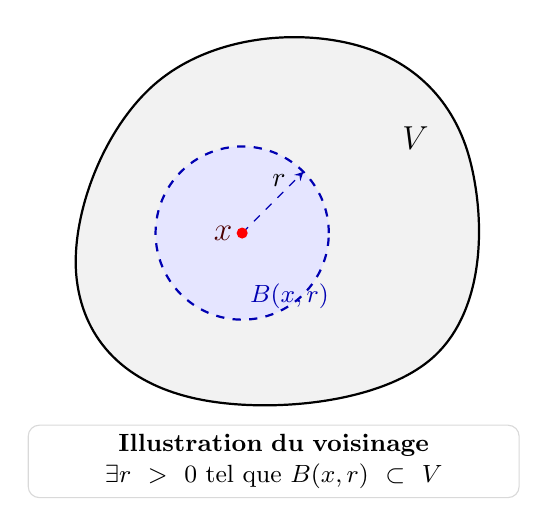
\begin{tikzpicture}[scale=1, >=stealth]

  % 1. Dessin de l'ensemble V (Voisinage) - Frontière continue
  \fill[gray!10] plot[smooth cycle, tension=0.7] coordinates {(-0.5,2) (2,2.5) (3.5,1) (3,-1.5) (0,-2) (-1.5,-0.5)};
  \draw[black, thick] plot[smooth cycle, tension=0.7] coordinates {(-0.5,2) (2,2.5) (3.5,1) (3,-1.5) (0,-2) (-1.5,-0.5)};
  \node[black] at (2.8, 1.3) {\large $V$};

  % 2. Placement du point x (centre de la boule)
  \coordinate (X) at (0.6, 0.1);
  
  % 3. Dessin de la boule ouverte B(x,r)
  % On utilise un cercle parfait pour représenter graphiquement la boule métrique
  \fill[blue!10] (X) circle (1.1cm);
  \draw[blue!70!black, thick, dashed] (X) circle (1.1cm);
  
  % Affichage du rayon r
  \draw[blue!70!black, ->, dashed] (X) -- node[above, pos=0.6, black] {$r$} +(45:1.1cm);
  
  % Nom de la boule
  \node[blue!70!black] at (1.2, -0.7) {\small $B(x,r)$};

  % Repère du point x
  \fill[red] (X) circle (2pt) node[left, red!30!black] {\large $x$};

  % 4. Légende descriptive en bas
  \node[text width=6cm, align=center, font=\small, draw=gray!30, rounded corners, fill=white] at (1,-2.8) {
    \textbf{Illustration du voisinage} \\
    $\exists r > 0 \text{ tel que } B(x,r) \subset V$
  };

\end{tikzpicture}
\end{center}

\remark{On notera $\mathcal{V}(x)$ l'ensemble des voisinages de $x$.}

\theorem{Proposition}{Propriétés des voisinages}{false}{
    \begin{enumerate}
        \item Tout voisinage de $x$ contient $x$. 
        \item $\bigcap_{V \in \mathcal{V}(x)} V = \{x\}$.
        \item L'intersection de deux voisinages de $x$ est un voisinage de $x$.
    \end{enumerate}
}

\training{Démontrer la proposition précédente}
\noindent\carreaux{10}

\theorem{Proposition}{Conséquence de l'équivalence des normes}{false}{
    Soient $\| \cdot \|_a$ et $\| \cdot \|_b$ deux normes équivalentes sur $E$. Alors pour tout $x \in E$, les ensembles des voisinages de $x$ pour les deux normes sont identiques, c'est-à-dire :
    $$\mathcal{V}_a(x) = \mathcal{V}_b(x).$$
    En particulier, en dimension finie, le choix de la norme n'affecte pas la notion de voisinage.
}


\section{Suites et limites}

\subsection{Généralités sur les suites}
\definition{
    Soit $A \subset E$. Une \textbf{suite} d'éléments de $A$ est une application $k \in \mathbb{N} \mapsto x_k \in A$, souvent notée $(x_k)_{k \in \mathbb{N}}$.
}

\definition{
    On dit d'une suite $(x_k)_{k \in \mathbb{N}}$ qu'elle est \textbf{bornée} s'il existe $r > 0$ tel que $\forall k \in \mathbb{N}, x_k \in B(0,r)$.
}

\subsection{Convergence des suites}

\definition{
    
    Soit $(x_n)_{n \in \mathbb{N}}$ une suite d'éléments de $E$. On dit que $(x_n)_{n \in \mathbb{N}}$ \textbf{converge} vers un élément $l \in E$ si :
    $$\forall \varepsilon > 0, \exists N \in \mathbb{N}, \forall n \geq N, \|x_n - l\| < \varepsilon.$$
    Dans ce cas, on écrit $\lim_{n \to +\infty} x_n = l$ ou $x_n \to l$.
}

\remark{De manière équivalente, on peut dire que $(x_n)_{n \in \mathbb{N}}$ converge vers $l$ :
\begin{itemize}
    \item si $\lim_{n \to +\infty} \|x_n - l\| = 0$.
    \item si $\forall \varepsilon > 0, \exists N \in \mathbb{N}, \forall n \geq N, x_n \in B(l,\varepsilon)$.
\end{itemize}}

\attention{ convergence dépend de la norme choisie. Ainsi, une suite peut converger pour une norme et ne pas converger pour une autre norme (sauf en dimension finie, vous l'aurez compris).}

\theorem{Proposition}{Convergence et équivalence des normes}{false}{
    Soient $\| \cdot \|_a$ et $\| \cdot \|_b$ deux normes équivalentes sur $E$. Alors une suite $(x_n)_{n \in \mathbb{N}}$ converge pour la norme $\| \cdot \|_a$ vers $l$ si, et seulement si, elle converge pour la norme $\| \cdot \|_b$ vers $l$.
}
\ndlr{cf. Laurent pour la preuve.}

\training{Montrer que la suite $(x_n)_{n \in \mathbb{N}}$ définie par $x_n = (\frac{1}{n}, 1 - \frac{1}{n})$ converge vers $(0,1)$ selon les normes $1$, $2$ et $\infty$ sur $\mathbb{R}^2$.}
\noindent \carreaux{6}

\training{Montrer que la suite de fonctions $(f_n)_{n \in \mathbb{N}}$ définie par $f_n(t) = t^n$ converge pour la norme $1$ vers la limite $f(t) = 0$, mais pas pour la norme $\infty$.}
\noindent \carreaux{4}

\remark{Dans le cas d'espaces vectoriels normés de dimension finie, par équivalence des normes, la convergence d'une suite ne dépend pas de la norme choisie. }

\theorem{Proposition}{Unicité de la limite}{false}{
    Soit $(x_n)_{n \in \mathbb{N}}$ une suite d'éléments de $E$. Si $(x_n)_{n \in \mathbb{N}}$ converge vers $l_1$ et $l_2$, alors $l_1 = l_2$.
}
\noindent{\textbf{Preuve :} Soit $\varepsilon > 0$.\\
Considérons $N_\epsilon$ tel que $$\| x_k - l_1 \| < \varepsilon/2 \text{ et } \| x_k - l_2 \| < \varepsilon/2 \text{ pour tout } k \ge N_\epsilon.$$
On remarque que $N_\varepsilon$ existe car $(x_n)_{n \in \mathbb{N}}$ converge. Par l'inégalité triangulaire, on a :
$$ \| l_1 - l_2 \| = \| l_1 - x_k + x_k - l_2 \| \le \| l_1 - x_k \| + \| x_k - l_2 \| < \frac{\varepsilon}{2} + \frac{\varepsilon}{2} = \varepsilon.$$
et comme $\varepsilon$ est arbitraire, on en déduit que $l_1 = l_2$. $ \hfill \square$
}

\theorem{Proposition}{}{false}{
    Toute suite convergente est bornée.
}
\noindent\textbf{Preuve :} Soit $\{x_k\}$ une suite convergente vers $l$. Posons $\varepsilon = 1$, il existe $N \in \mathbb{N}$ tel que $x_k \in B(l, 1)$ pour tout $k \ge N$. L'ensemble des vecteurs $\{x_0, x_1, \dots, x_{N-1}\}$ est fini, et on peut poser $r = \max_{k < N} \|x_k\| < +\infty$. En posant maintenant $R = \max(r + 1, \|l\| + 1)$, on a la dichotomie
\begin{itemize}
    \item si $k < N$, $\|x_k\| < r + 1 \le R$;
    \item si $k \ge N$, $\|x_k\| = \|x_k - l + l\| \le \|x_k - l\| + \|l\| \le 1 + \|l\| \le R$.
\end{itemize}
Dans les deux cas on conclut que $x_k \in B(0, R)$. \hfill $\square$

\theorem{Proposition}{Convergence des suites et des suites extraites}{false}{
    Toute sous-suite d'une suite convergente converge vers la même limite.
}
\noindent\textbf{Preuve :} Soit $\{x_k\}_{k \in \mathbb{N}}$ une suite convergente vers la limite $x \in E$. Alors
$$\forall \varepsilon > 0, \exists N \in \mathbb{N} : \forall k \ge N, \|x_k - x\| < \varepsilon.$$
Soit $\{x_{\varphi(k)}\}_{k \in \mathbb{N}}$ une sous-suite, puisque $\varphi$ est monotone strictement croissante, $\varphi(n) \ge n$, on en déduit que
$$\forall \varepsilon > 0, \exists N \in \mathbb{N} : \forall k \ge N, \|x_{\varphi(k)} - x\| < \varepsilon$$
ce qui implique que $x_{\varphi(k)} \to x$. \hfill $\square$

\theorem{Proposition}{Linéarité de la limite}{false}{
    Soient $(x_n)_{n \in \mathbb{N}}$ et $(y_n)_{n \in \mathbb{N}}$ deux suites convergentes vers $x$ et $y$ respectivement. Alors pour tout $\alpha, \beta \in \mathbb{R}$, la suite $(\alpha x_n + \beta y_n)_{n \in \mathbb{N}}$ converge vers $\alpha x + \beta y$.
}

\training{Montrer la proposition précédente.}
\noindent \carreaux{6}

\subsection{Convergence et suites extraites}

\definition{
    Soit $A \subset E$ et soit $(x_k)_{k \in \mathbb{N}}$ une suite d'éléments de $A$.\\
    Une \textbf{suite extraite} de $(x_k)_{k \in \mathbb{N}}$ est une suite $(x_{\phi(k)})_{k \in \mathbb{N}}$ où $\phi : \mathbb{N} \to \mathbb{N}$ est une application strictement croissante.
}

\example{
    Soit $(x_k)_{k \in \mathbb{N}}$ la suite définie par $x_k = (-1)^k$. Alors $(x_{2k})_{k \in \mathbb{N}}$ est une suite extraite de $(x_k)_{k \in \mathbb{N}}$, et elle est constante égale à $1$.
}

\theorem{Proposition}{Caractérisation de la convergence par les suites extraites}{false}{
    Soit $(x_k)_{k \in \mathbb{N}}$ une suite d'éléments de $E$. Alors $(x_k)_{k \in \mathbb{N}}$ converge vers $l$ si et seulement si toute suite extraite de $(x_k)_{k \in \mathbb{N}}$ converge vers $l$.
}

\remark{En particulier, si une suite admet deux sous-suites convergeant vers des limites différentes, alors la suite n'est pas convergente.}

\subsection{Topologie et suites}

\theorem{Proposition}{Convergence et adhérence}{false}{
    Soit $A \subset E$. Alors $a \in \overline{A}$ si et seulement si il existe une suite $(x_n)_{n \in \mathbb{N}}$ d'éléments de $A$ qui converge vers $a$.
}
\noindent\textbf{Preuve :} \\
$\Rightarrow/$ Pour tout $\varepsilon > 0$ $B(a,\varepsilon) \cap \{x_k\}_k \neq \varnothing$ par la remarque sur les définitions équivalentes de la convergence. Par le lemme sur les propriétés de l'intérieur et de l'adhérence, on a que $a \in \overline{A}$. \\[0.5em]
$\Leftarrow/$ Pour tout $k \in \mathbb{N}$ posons $\varepsilon = \frac{1}{k}$, par le même lemme $B(a,1/k) \cap A \neq \varnothing$ et posons $x_k$ élément quelconque de $B(a,1/k) \cap A$. Alors la suite construite $\{x_k\}_k \subset A$ et $x_k \to a$. \hfill $\square$

\theorem{Proposition}{Caractérisation des fermés par les suites}{false}{
    Soit $F \subset E$. Alors $F$ est fermé si et seulement si pour toute suite $(x_n)_{n \in \mathbb{N}}$ d'éléments de $F$ qui converge vers un élément $x \in E$, on a $x \in F$.
}

\training{Montrer que $B(0,1) \setminus \{0\}$ est ouvert et que $\overline{B}(0,1) \setminus \{0\}$ n'est ni ouvert, ni fermé.}
\noindent \carreaux{10}

\section{Topologie des espaces vectoriels normés}
\subsection{Adhérence}

\definition{
    Soit $a \in E$ et soit $A \subset E$. On dit que $a$ est un \textbf{point adhérent} à $A$ si pour tout $\varepsilon > 0$, la boule ouverte $B(a,\varepsilon)$ contient au moins un point de $A$. Autrement dit,
    $$\forall \varepsilon > 0, B(a,\varepsilon) \cap A \neq \varnothing.$$
}

\example{$1$ est adhérent à $[0,1[$, $0$ est adhérent à $]0,1]$.}

\theorem{Théorème}{Caractérisation de l'adhérence par les suites}{false}{
    Soient $A \subset E$ et $a \in E$. Alors :
    $$a \in \overline{A} \Leftrightarrow \exists (x_n)_{n \in \mathbb{N}} \subset A, x_n \to a$$
}
\ndlr{cf. Laurent pour la preuve.}

\definition{
    Soit $A \subset E$. On appelle \textbf{adhérence} de $A$ et on note $\overline{A}$ l'intersection de tous les fermés contenant $A$. On a :
    $$ \overline{A} = \bigcap \{ F \supset A \mid F \text{ est un fermé de } E \} $$
    C'est le plus petit fermé contenant $A$.
}

\begin{center}
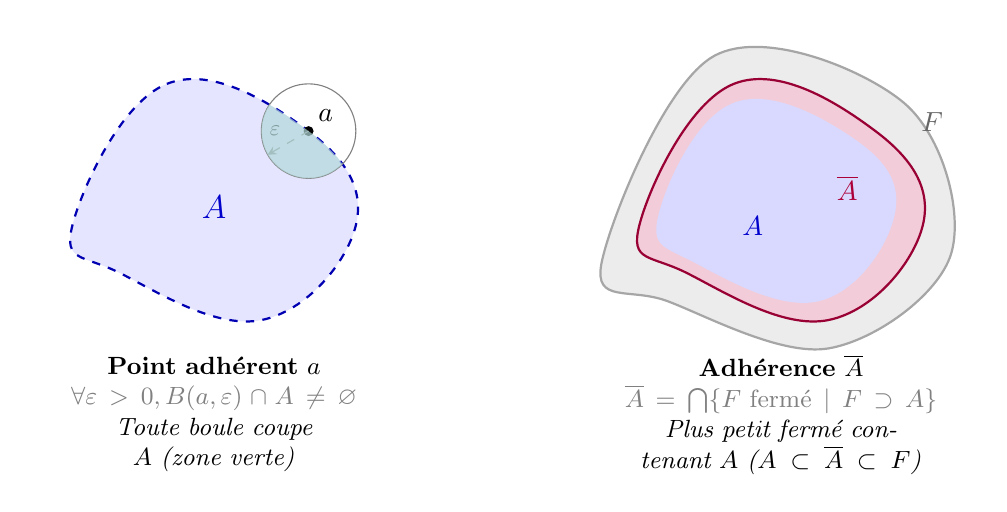
\begin{tikzpicture}[scale=1.2, >=stealth]

  % ==========================================
  % SECTION 1 : POINT ADHÉRENT (À GAUCHE)
  % ==========================================
  \begin{scope}[shift={(0,0)}]
    % Remplissage de l'ensemble A
    \fill[blue!10] plot[smooth cycle, tension=0.7] coordinates {(0,0) (1,1.5) (2.5,1) (3,0) (2,-1) (0.5,-0.5)};
    
    % Frontière de A en pointillés (A peut être ouvert ou quelconque)
    \draw[blue!70!black, thick, dashed] plot[smooth cycle, tension=0.7] coordinates {(0,0) (1,1.5) (2.5,1) (3,0) (2,-1) (0.5,-0.5)};
    
    % Nom de l'ensemble
    \node[blue!80!black] at (1.5, 0.2) {\large $A$};
    
    % Point adhérent a (situé sur le bord de A)
    \coordinate (A_point) at (2.5, 1);
    \fill[black] (A_point) circle (1.5pt) node[above right] {$a$};
    
    % Boule ouverte centrée en a qui croise A
    \draw[gray, thin] (A_point) circle (0.5cm);
    \draw[dashed, ->, gray] (A_point) -- node[above left, scale=0.8, black] {$\varepsilon$} +(210:0.5cm);
    
    % Zone d'intersection B(a, eps) \cap A
    \begin{scope}
      \clip plot[smooth cycle, tension=0.7] coordinates {(0,0) (1,1.5) (2.5,1) (3,0) (2,-1) (0.5,-0.5)};
      \fill[teal!30, opacity=0.7] (A_point) circle (0.5cm);
    \end{scope};
    
    % Légende sous la première figure
    \node[text width=4.5cm, align=center, font=\small] at (1.5,-2) {
      \textbf{Point adhérent $a$}\\
      \textcolor{gray}{$\forall \varepsilon > 0, B(a,\varepsilon) \cap A \neq \varnothing$}\\
      \textit{Toute boule coupe $A$ (zone verte)}
    };
  \end{scope}

  % ==========================================
  % SECTION 2 : ADHÉRENCE \overline{A} (À DROITE)
  % ==========================================
  \begin{scope}[shift={(6,0)}]
    % Fermé F englobant (en gris clair)
    \fill[gray!15] plot[smooth cycle, tension=0.6] coordinates {(-0.4,-0.4) (0.8,1.8) (2.8,1.3) (3.3,-0.3) (2,-1.3) (0.3,-0.8)};
    \draw[gray!70, thick] plot[smooth cycle, tension=0.6] coordinates {(-0.4,-0.4) (0.8,1.8) (2.8,1.3) (3.3,-0.3) (2,-1.3) (0.3,-0.8)};
    \node[gray!80!black] at (3.1, 1.1) {$F$};

    % Remplissage de l'adhérence \overline{A}
    \fill[purple!20] plot[smooth cycle, tension=0.7] coordinates {(0,0) (1,1.5) (2.5,1) (3,0) (2,-1) (0.5,-0.5)};
    
    % Frontière FERMÉE de \overline{A} (trait plein violet)
    \draw[purple!80!black, thick] plot[smooth cycle, tension=0.7] coordinates {(0,0) (1,1.5) (2.5,1) (3,0) (2,-1) (0.5,-0.5)};
    
    % Intérieur de A (en bleu très clair)
    \fill[blue!15] plot[smooth cycle, tension=0.7] coordinates {(0.2,0.1) (1,1.3) (2.3,0.9) (2.7,0.1) (1.9,-0.8) (0.6,-0.4)};
    \node[blue!80!black] at (1.2, 0) {$A$};
    \node[purple!90!black] at (2.2, 0.4) {$\overline{A}$};
    
    % Légende sous la deuxième figure
    \node[text width=4.8cm, align=center, font=\small] at (1.5,-2) {
      \textbf{Adhérence $\overline{A}$}\\
      \textcolor{gray}{$\overline{A} = \bigcap \{ F \text{ fermé} \mid F \supset A \}$}\\
      \textit{Plus petit fermé contenant $A$ ($A \subset \overline{A} \subset F$)}
    };
  \end{scope}

\end{tikzpicture}
\end{center}


\subsection{Intérieur}

\definition{
    Soit $a \in E$ et soit $A \subset E$. On dit que $a$ est un \textbf{point intérieur} à $A$ si il existe $\varepsilon > 0$ tel que la boule ouverte $B(a,\varepsilon)$ est contenue dans $A$. Autrement dit,
    $$\exists \varepsilon > 0, B(a,\varepsilon) \subset A.$$
}

\example{Tout point de $]0,1[$ est un point intérieur à $]0,1[$. Aucun point de $[0,1]$ n'est un point intérieur à $[0,1]$.}

\definition{
    Soit $A \subset E$. On appelle \textbf{intérieur} de $A$ et on note $\overset{\circ}{A}$ l'union de tous les ouverts contenus dans $A$. On a :
    $$ \overset{\circ}{A} = \bigcup \{ U \subset A \mid U \text{ est un ouvert de } E \} $$
    C'est le plus grand ouvert contenu dans $A$.
}

\definition{
    Soit $A \subset E$. On appelle \textbf{frontière} de $A$ et on note $\partial A$ la différence entre l'adhérence et l'intérieur de $A$. On a :
    $$ \partial A = \overline{A} \setminus \overset{\circ}{A} $$
}

\begin{center}
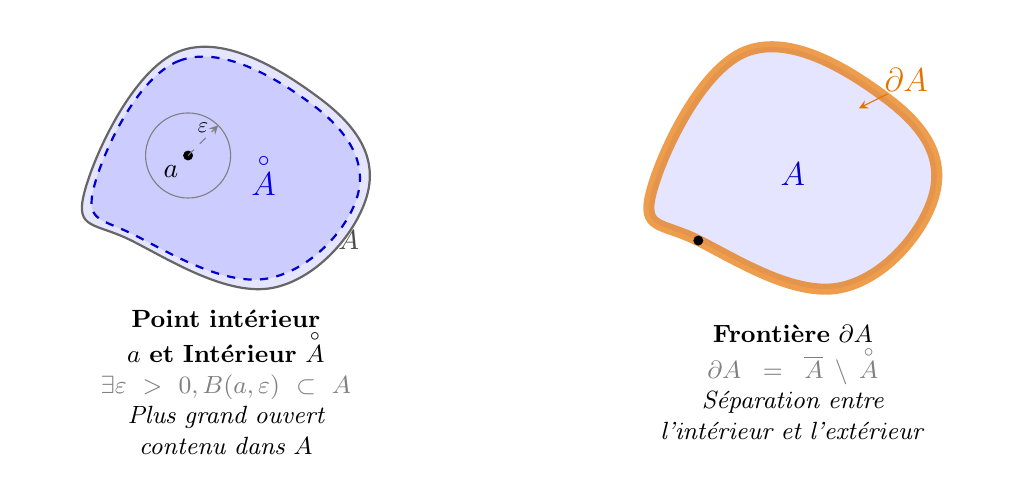
\begin{tikzpicture}[scale=1.2, >=stealth]

  % ==========================================
  % SECTION 1 : POINT INTÉRIEUR & INTÉRIEUR (À GAUCHE)
  % ==========================================
  \begin{scope}[shift={(0,0)}]
    % Ensemble A global (avec sa frontière réelle en trait plein)
    \fill[blue!10] plot[smooth cycle, tension=0.7] coordinates {(0,0) (1,1.5) (2.5,1) (3,0) (2,-1) (0.5,-0.5)};
    \draw[black!60, thick] plot[smooth cycle, tension=0.7] coordinates {(0,0) (1,1.5) (2.5,1) (3,0) (2,-1) (0.5,-0.5)};
    
    % Intérieur \overset{\circ}{A} (zone bleue avec bord en pointillés)
    \fill[blue!20] plot[smooth cycle, tension=0.7] coordinates {(0.1,0.05) (1,1.4) (2.4,0.95) (2.9,0) (1.95,-0.9) (0.55,-0.45)};
    \draw[blue!80!black, thick, dashed] plot[smooth cycle, tension=0.7] coordinates {(0.1,0.05) (1,1.4) (2.4,0.95) (2.9,0) (1.95,-0.9) (0.55,-0.45)};
    
    % Noms des ensembles
    \node[blue!90!black] at (1.9, 0.2) {\large $\overset{\circ}{A}$};
    \node[black!70] at (2.8, -0.5) {$A$};

    % Point intérieur a
    \coordinate (A_int) at (1.1, 0.4);
    \fill[black] (A_int) circle (1.5pt) node[below left] {$a$};
    
    % Boule entièrement contenue dans A
    \draw[gray, thin] (A_int) circle (0.45cm);
    \draw[dashed, ->, gray] (A_int) -- node[above, scale=0.8, black] {$\varepsilon$} +(45:0.45cm);

    % Légende sous la première figure
    \node[text width=4.8cm, align=center, font=\small] at (1.5,-2) {
      \textbf{Point intérieur $a$ et Intérieur $\overset{\circ}{A}$}\\
      \textcolor{gray}{$\exists \varepsilon > 0, B(a,\varepsilon) \subset A$}\\
      \textit{Plus grand ouvert contenu dans $A$}
    };
  \end{scope};

  % ==========================================
  % SECTION 2 : FRONTIÈRE \partial A (À DROITE)
  % ==========================================
  \begin{scope}[shift={(6,0)}]
    % Remplissage léger de l'ensemble A
    \fill[blue!10] plot[smooth cycle, tension=0.7] coordinates {(0,0) (1,1.5) (2.5,1) (3,0) (2,-1) (0.5,-0.5)};
    \node[blue!80!black] at (1.5, 0.2) {\large $A$};

    % Épaisseur matérialisant la frontière \partial A = \overline{A} \setminus \overset{\circ}{A}
    \draw[orange!90!black, line width=4pt, opacity=0.7] plot[smooth cycle, tension=0.7] coordinates {(0,0) (1,1.5) (2.5,1) (3,0) (2,-1) (0.5,-0.5)};
    
    % Indication du nom de la frontière
    \node[orange!90!black] at (2.7, 1.2) {\large $\partial A$};
    \draw[->, orange!90!black, thin] (2.5, 1.05) -- (2.2, 0.9);

    % Point sur la frontière
    \coordinate (A_front) at (0.5, -0.5);
    \fill[black] (A_front) circle (1.5pt);

    % Légende sous la deuxième figure
    \node[text width=4.8cm, align=center, font=\small] at (1.5,-2) {
      \textbf{Frontière $\partial A$}\\
      \textcolor{gray}{$\partial A = \overline{A} \setminus \overset{\circ}{A}$}\\
      \textit{Séparation entre l'intérieur et l'extérieur}
    };
  \end{scope}

\end{tikzpicture}
\end{center}

\example{
    Soit $A = (0,1) \subset \mathbb{R}$. Alors :
    \begin{itemize}
        \item $\overset{\circ}{A} = ]0,1[$,
        \item $\overline{A} = [0,1]$,
        \item $\partial A = \{0,1\}$.
    \end{itemize}
}

\theorem{Lemme}{Propriétés de l'intérieur et de l'adhérence}{false}{
    Soit $A \subset E$. Alors :
    \begin{enumerate}
        \item $\overset{\circ}{A} \subset A \subset \overline{A}$,
        \item si $A$ est ouvert, alors $\overset{\circ}{A} = A$,
        \item si $A$ est fermé, alors $\overline{A} = A$,
    \end{enumerate}
}

\training{Montrer les propriétés de l'intérieur et de l'adhérence.}
\noindent \carreaux{12}

\subsection{Ouverts}
\definition{Soit $A \subset E$. On dit que $A$ est un \textbf{ouvert} si pour tout $x \in A$, il existe $r > 0$ tel que $B(x,r) \subset A$.}
\vocabulary{On appelle \textbf{topologie} et on note $\mathcal{T}_{\| \cdot \|}$ sur $E$ l'ensemble des ouverts de $E$ pour la norme $\| \cdot \|$.}

\remark{Autrement dit, $A$ est ouvert si et seulement si $A = \overset{\circ}{A}$.}

\theorem{Proposition}{Équivalence des normes}{false}{
    Soient $\| \cdot \|_a$ et $\| \cdot \|_b$ deux normes sur $E$. Supposons que ces deux normes sont équivalentes.\\
    Alors un sous-ensemble $A \subset E$ est ouvert pour la norme $\| \cdot \|_a$ si et seulement si il est ouvert pour la norme $\| \cdot \|_b$.
}
\begin{center}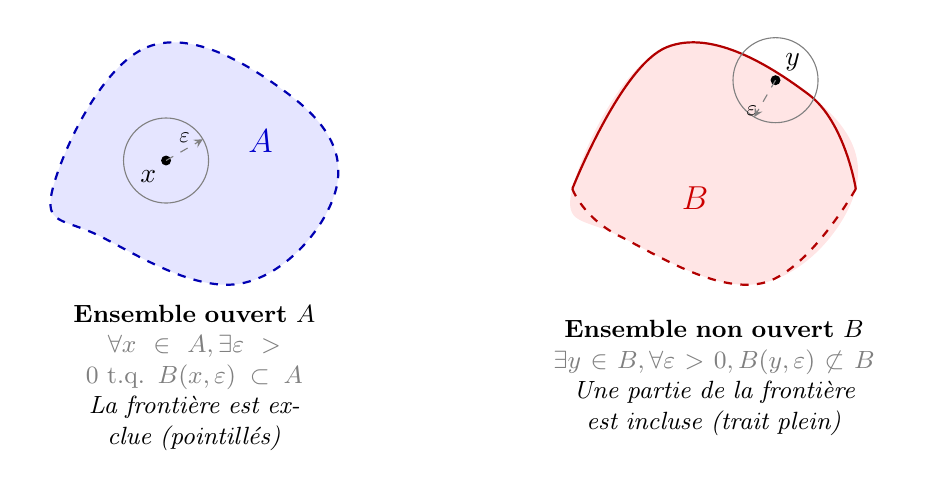
\begin{tikzpicture}[scale=1.2, >=stealth]

  % ==========================================
  % SECTION 1 : ENSEMBLE OUVERT (À GAUCHE)
  % ==========================================
  \begin{scope}[shift={(0,0)}]
    % Remplissage de l'ensemble ouvert
    \fill[blue!10] plot[smooth cycle, tension=0.7] coordinates {(0,0) (1,1.5) (2.5,1) (3,0) (2,-1) (0.5,-0.5)};
    
    % Frontière en pointillés (indique que le bord est exclu)
    \draw[blue!70!black, thick, dashed] plot[smooth cycle, tension=0.7] coordinates {(0,0) (1,1.5) (2.5,1) (3,0) (2,-1) (0.5,-0.5)};
    
    % Nom de l'ensemble
    \node[blue!80!black] at (2.2, 0.5) {\large $A$};
    
    % Point intérieur x
    \coordinate (X) at (1.2, 0.3);
    \fill[black] (X) circle (1.5pt) node[below left] {$x$};
    
    % Boule ouverte centrée en x et incluse dans A
    \draw[gray, thin] (X) circle (0.45cm);
    \draw[dashed, ->, gray] (X) -- node[above, scale=0.8, black] {$\varepsilon$} +(30:0.45cm);
    
    % Légende sous la première figure
    \node[text width=4cm, align=center, font=\small] at (1.5,-2) {
      \textbf{Ensemble ouvert $A$}\\
      \textcolor{gray}{$\forall x \in A, \exists \varepsilon > 0 \text{ t.q. } B(x,\varepsilon) \subset A$}\\
      \textit{La frontière est exclue (pointillés)}
    };
  \end{scope}

  % ==========================================
  % SECTION 2 : ENSEMBLE NON OUVERT (À DROITE)
  % ==========================================
  \begin{scope}[shift={(5.5,0)}]
    % Remplissage de l'ensemble non ouvert
    \fill[red!10] plot[smooth cycle, tension=0.7] coordinates {(0,0) (1,1.5) (2.5,1) (3,0) (2,-1) (0.5,-0.5)};
    
    % Frontière hybride : une partie fermée (trait plein) et une partie ouverte (pointillés)
    % On découpe le contour pour illustrer un bord adhérent
    \draw[red!70!black, thick] plot[smooth, tension=0.7] coordinates {(0,0) (1,1.5) (2.5,1) (3,0)};
    \draw[red!70!black, thick, dashed] plot[smooth, tension=0.7] coordinates {(3,0) (2,-1) (0.5,-0.5) (0,0)};
    
    % Nom de l'ensemble
    \node[red!80!black] at (1.3, -0.1) {\large $B$};
    
    % Point y sur la frontière incluse
    \coordinate (Y) at (2.15, 1.15); % Point situé sur la ligne continue supérieure
    \fill[black] (Y) circle (1.5pt) node[above right] {$y$};
    
    % Boule centrée en y (qui sort forcément de l'ensemble)
    \draw[gray, thin] (Y) circle (0.45cm);
    \draw[dashed, ->, gray] (Y) -- node[below left, scale=0.8, black] {$\varepsilon$} +(-120:0.45cm);
    
    % Légende sous la deuxième figure
    \node[text width=4.5cm, align=center, font=\small] at (1.5,-2) {
      \textbf{Ensemble non ouvert $B$}\\
      \textcolor{gray}{$\exists y \in B, \forall \varepsilon > 0, B(y,\varepsilon) \not\subset B$}\\
      \textit{Une partie de la frontière est incluse (trait plein)}
    };
  \end{scope}

\end{tikzpicture}
\end{center}

\remark{On en déduit que les ouverts dans $\mathbb{R}^n$ sont les mêmes pour toutes les normes équivalentes.}

\theorem{Proposition}{Boule ouverte et ouvert}{false}{
    Soit $\| \cdot \|$ une norme sur $E$. Alors toute boule ouverte est un ouvert de $E$.
}
\noindent\textbf{Preuve :} Soit $y \in B(x,R)$, en particulier $\|y - x\| < R$. On a que $B(y, R - \|y - x\|) \subset B(x,R)$. En effet, soit $z \in B(y, R - \|y - x\|)$. Alors, par l'inégalité triangulaire,
$$\|z - x\| = \|z - y + y - x\| \le \|z - y\| + \|y - x\| < R - \|y - x\| + \|y - x\| = R \implies z \in B(x,R).$$
$ \hfill \square$


\theorem{Proposition}{Union et intersection d'ouverts}{false}{
    Soit $\| \cdot \|$ une norme sur $E$. Alors :
    \begin{enumerate}
        \item L'union d'une famille quelconque d'ouverts est un ouvert.
        \item L'intersection d'une famille finie d'ouverts est un ouvert.
    \end{enumerate}
}
\attention{L'intersection d'une famille infinie d'ouverts n'est pas nécessairement un ouvert : par exemple, dans $\mathbb{R}$, l'intersection des ouverts $(-\frac{1}{n}, \frac{1}{n})$ pour $n \in \mathbb{N}^*$ est $\{0\}$, qui n'est pas un ouvert.}

\training{Montrer la proposition précédente.}
\noindent \carreaux{7}

\theorem{Proposition}{}{false}{
    Soit $A \subset E$. Alors $A$ est ouvert si et seulement si $A = \overset{\circ}{A}$.
}

\subsection{Fermés}

\definition{
    Soit $F \subset E$. On dit que $F$ est un \textbf{fermé} si son complémentaire $E \setminus F$ est un ouvert.
}

\theorem{Proposition}{Boule fermée et fermé}{false}{
    Soit $\| \cdot \|$ une norme sur $E$. Alors toute boule fermée est un fermé de $E$.
}

\training{Montrer la proposition précédente.}
\noindent \carreaux{7}

\theorem{Proposition}{Union et intersection de fermés}{false}{
    Soit $\| \cdot \|$ une norme sur $E$. Alors :
    \begin{enumerate}
        \item L'intersection d'une famille quelconque de fermés est un fermé.
        \item L'union d'une famille finie de fermés est un fermé.
    \end{enumerate}
}

\remark{Il est important de noter qu'il existe des ensembles qui ne sont ni ouverts ni fermés, ainsi que des ensembles qui sont à la fois ouverts et fermés (appelés \textit{ouverts-fermés}).}

\theorem{Proposition}{}{false}{
    Soit $A \subset E$. Alors $A$ est fermé si et seulement si $A = \overline{A}$.
}

\theorem{Théorème}{Caractérisation séquentielle des fermés}{false}{
    Soit $F \subset E$. Alors $F$ est fermé si et seulement si pour toute suite $(x_n)_{n \in \mathbb{N}}$ d'éléments de $F$ qui converge vers un élément $x \in E$, on a $x \in F$.
}

\theorem{Proposition}{Équivalence sur les voisinages}{false}{
    Soit $A \subset E$.
    \begin{enumerate}
        \item $A$ est un ouvert $\iff \forall x \in A, A \in \mathcal{V}(x)$ \textit{(c'est-à-dire que $A$ est un voisinage de chacun de ses points)},
        \item $A$ est un voisinage de $x \iff x \in \overset{\circ}{A}$.
    \end{enumerate}
}
\ndlr{cf. Laurent pour la preuve}

\theorem{Théorème}{Parties ouverts-fermés d'un evn}{true}{
    Soit $E$ un espace vectoriel normé. Alors les seuls sous-ensembles de $E$ qui sont à la fois ouverts et fermés sont $\varnothing$ et $E$ lui-même.
}

\section{Limite de fonctions}

Dans section section, $(E, \|\cdot\|)$ et $(F, \|\cdot\|_F)$ sont deux espaces vectoriels normés.

\definition{
    Soit $a$ un point adhérent à une partie non vide $A$ de $E$ et $f : A \to F$ une application. On dit que $f(x)$ tend vers $\ell \in F$ quand $x$ tend vers $a$ si, quelque soit $(x_n)_{n \geq 1}$ une suite d'éléments de $A$ on a
    \[
        x_n \xrightarrow[n \to +\infty]{\|\cdot\|_E} a \implies f(x_n) \xrightarrow[n \to +\infty]{\|\cdot\|_F} \ell.
    \]
    Dans ce cas, cet élément $\ell$ est unique, s'appelle la limite de la fonction $f$ quand $x$ tend vers $a$ et on écrit,
    \[
        f(x) \xrightarrow[x \to a]{} \ell \quad \text{ou} \quad \lim_{x \to a} f(x) = \ell.
    \]
}

\remark{
    On rappelle que si $E$ est de dimension finie cette notion de limite ne dépend pas du choix de la norme utilisée puisque toutes les normes sont équivalentes en dimension finie.
}

\example{
    \begin{enumerate}
        \item Soit $f : \mathbb{R}^2 \to \mathbb{R}$ définie par $f(x,y) = x^2 y^3$. Alors $\lim_{(x,y) \to (1,2)} f(x,y) = 8$. En effet, supposons que $(x_n, y_n) \xrightarrow[n \to +\infty]{} (1,2)$. Alors $x_n \xrightarrow[n \to +\infty]{} 1$ et $y_n \xrightarrow[n \to +\infty]{} 2$. Ainsi $x_n^2 \xrightarrow[n \to +\infty]{} 1$ et $y_n^3 \xrightarrow[n \to +\infty]{} 8$. Finalement, $x_n^2 y_n^3 \xrightarrow[n \to +\infty]{} 8$.
        \item Soit $E$ un espace préhilbertien et $u \in E$ et $\ell_u : v \mapsto \langle u,v \rangle$. Calculer $\lim_{v \to 0} \ell_u(v)$.\\
        Soit $(v_n)_{n \in \mathbb{N}}$ une suite de $E$ qui converge vers $0$ dans $E$. On a, pour tout $n \in \mathbb{N}$
        \[
            |\ell_u(0) - \ell_u(v_n)| = |\langle u,0 \rangle - \langle u,v_n \rangle| = |\langle u,v_n \rangle| \leq \|u\| \cdot \|v_n\| \xrightarrow[n \to +\infty]{} 0
        \]
        Donc $\langle u,v_n \rangle \xrightarrow[n \to +\infty]{} 0$.
    \end{enumerate}
}

\theorem{Proposition}{Linéarité et produit de limites}{false}{
    Soient $f,g : A \to F$ deux applications et $a$ un point adhérent à $A$. Supposons que $\lim_{x \to a} f(x) = \ell_f$ et $\lim_{x \to a} g(x) = \ell_g$. Alors :
    \begin{enumerate}
        \item Pour tout $\alpha, \beta \in \mathbb{R}$, $\lim_{x \to a} (\alpha f(x) + \beta g(x)) = \alpha \ell_f + \beta \ell_g$.
        \item Si $F = \mathbb{K}$, alors $\lim_{x \to a} f(x) g(x) = \ell_f \ell_g$.
    \end{enumerate}
}

\noindent{\textbf{Preuve :} Suit immédiatement des mêmes propriétés concernant les suites.}


\theorem{Proposition}{Composition de limites}{false}{
    Soit $a$ un point adhérent à une partie non vide $A$ de $E$ et $f,g : A \to F$ deux applications. Soit $B$ une partie d'un espace vectoriel normé $G$ et $h : B \to G$ avec $f(A) \subset B$ et $\ell$ un point adhérent à $B$. Supposons que $f(x)$ tend vers $\ell \in F$ quand $x$ tend vers $a$ et $h(y)$ tend vers $\ell' \in G$ quand $y$ tend vers $\ell$ alors $h(f(x))$ tend vers $\ell'$ quand $x$ tend vers $a$.
}

\noindent{\textbf{Preuve :} Suit immédiatement des mêmes propriétés concernant les suites.}


\theorem{Proposition}{Limite et coordonnées dans une base}{false}{
    Soit $a$ un point adhérent à une partie $A$ de $E$ et $f : A \to F$ une application. Supposons que $F$ est de dimension finie et $\mathcal{B}$ une base de $F$. Alors $f$ admet une limite en $a$ si, et seulement si, les coordonnées de $f$ dans $\mathcal{B} = (e_1, \dots, e_m)$ admettent une limite en $a$. Dans ce cas, si $f(x) = f_1(x)e_1 + \dots + f_m(x)e_m$ alors on a :
    \[
        \lim_{x \to a} f(x) = \left( \lim_{x \to a} f_1(x) \right) e_1 + \dots + \left( \lim_{x \to a} f_m(x) \right) e_m.
    \]
}

\noindent{\textbf{Preuve :} Suit immédiatement des mêmes propriétés concernant les suites.}

\theorem{Théorème}{Caractérisation alternative de la limite d'une fonction}{false}{
    Soit $a$ un point adhérent à une partie non vide $A$ de $E$ et $f : A \to F$ une application. Alors $f(x)$ tend vers $\ell \in F$ quand $x$ tend vers $a$ si, et seulement si, pour tout $\varepsilon > 0$, il existe $\eta > 0$ tel que
    \[
        \forall x \in A, \|x - a\| < \eta \implies \|f(x) - \ell\| < \varepsilon.
    \]
}

\noindent{\textbf{Preuve :}
    \textbf{$\implies$)} Supposons 1) et montrons 2) par absurde. Pour cela supposons qu'il existe $\varepsilon > 0$, pour tout $\eta > 0$ il existe $x_\eta \in A$ tel que
    \[
        \|x_\eta - a\|_E \leq \eta \quad \text{et} \quad \|f(x_\eta) - \ell\|_F \geq \varepsilon.
    \]
    En particulier, pour tout $n \geq 1$, il existe $x_n \in A$ tel que
    \[
        \|x_n - a\|_E \leq \frac{1}{n} \quad \text{et} \quad \|f(x_n) - \ell\|_F \geq \varepsilon.
    \]
    On a donc une suite de vecteurs $x_n \in A$ tendant vers $a$ et $f(x_n)$ ne tend pas vers $\ell$ quand $n$ tend vers l'infini, ce qui contredit l'hypothèse 1).

    \textbf{$\impliedby$)} Réciproquement, supposons 2) et montrons 1). Pour cela soit $x_n \in A$ qui tend vers $a$ quand $n$ tend vers l'infini. Soit $\varepsilon > 0$. Il existe $\eta > 0$ tel que
    \[
        \forall x \in A, \quad \|x - a\|_E \leq \eta \implies \|f(x) - \ell\|_F \leq \varepsilon,
    \]
    Pour ce $\eta$, il existe un entier naturel $N$, tel que
    \[
        \|x_n - a\|_E \leq \eta \quad \text{dès que } n \geq N.
    \]
    Par suite,
    \[
        \|f(x_n) - \ell\|_F \leq \varepsilon \quad \text{dès que } n \geq N.
    \]
    Ce qui montre que $f(x_n)$ converge vers $\ell$ quand $n$ tend vers l'infini.
}

\newpage
\tableofcontents
\section*{Crédits}
Ce cours provient du polycopié de cours de l'Université Paris Cité réalisé par Alessandro Zilio enrichi et modifié par mes soins à des fins pédagogiques. Assurez-vous de citer correctement la source si vous utilisez ce cours dans vos travaux.\\\\
Ce cours est mis à disposition selon les termes de la Licence Creative Commons \ccbyncsa\ \textbf{Attribution - Pas d'Utilisation Commerciale - Partage dans les Mêmes Conditions 4.0 International}. 
Pour voir une copie de cette licence, visitez \url{http://creativecommons.org/licenses/by-nc-sa/4.0/}.

\end{document}
